\documentclass[conference]{IEEEtran}
\usepackage[T1]{fontenc}
\usepackage{amsmath,amssymb,graphicx,booktabs,url}
\usepackage[hidelinks]{hyperref}
\newcommand{\pending}{\textit{Not measured}}
\title{Spine-Guided Solar Filament Segmentation\\with Native-Resolution Features and Temporal Validation}
\author{\IEEEauthorblockN{Arjun Vijay Prakash}
\IEEEauthorblockA{Independent Researcher}}
\begin{document}
\maketitle
\begin{abstract}
Solar filament segmentation requires preserving narrow structures despite illumination variation and atmospheric artifacts. This note describes an implemented pipeline for IEEE Big Data Cup 2026 Challenge 02. Radial normalization and contrast-limited adaptive histogram equalization precede native-resolution crop training with full-disk context. SegFormer-B3 and ConvNeXt-Small U-Net++ members combine a full-resolution branch with mask, skeleton, and boundary heads. Dice, focal, and differentiable centerline losses supervise shape and connectivity. Five-fold validation groups physical observations and temporally adjacent dates while retaining independent annotation views. Controlled tests reproduce the public organizer notebook's Panoptic Quality calculation; a multiscale grid-IoU diagnostic is separately labeled provisional. A synthetic import-to-submission smoke test verifies integration. % PILOT_ABSTRACT
The approved release contains 707 physical training images, 1154 annotation views, 8199 annotations, and 180 test images. Completed five-fold experiments obtain pooled reference PQ 0.3444 for ConvNeXt-Small U-Net++ and 0.1623 for SegFormer-B3, using default instance extraction without validation augmentation. Matched-budget fold-0 comparisons identify instance fragmentation as a remaining concern. An earlier development-model submission obtains public PQ 0.27; it is distinct from these five-fold experiments. With extraction frozen on fold 0, the two-backbone ensemble obtains reference PQ 0.3806 across all 905 annotation views in folds 1--4 without validation augmentation. Ten-member D4 test inference obtains public leaderboard PQ 0.33. A larger-crop refinement is complete but not selected.
% END_PILOT_ABSTRACT
\end{abstract}
\begin{IEEEkeywords}
solar filaments, H-alpha, instance segmentation, topology, temporal validation
\end{IEEEkeywords}

\section{Introduction}
Solar filament segmentation must retain thin extensions, distinguish nearby structures, and avoid atmospheric artifacts. MAGFiLO provides manually reviewed annotations for GONG H-alpha observations~\cite{magfilo}.

The competition requires precise boundaries and coherent instances~\cite{challenge}. The system predicts foreground, skeleton, and boundary maps to preserve narrow material while separating adjacent objects.

\section{Data and evaluation contracts}
\subsection{Observation identity and independent annotators}
The full MAGFiLO release contains 10,244 annotations associated with 1,593 annotator-image records; official dataset documentation identifies 958 unique observations~\cite{magfiloweb}. Thus 1,593 must not be interpreted as the number of independent physical images. Independent annotators may disagree about filament extent and whether nearby pieces form one object. The pipeline retains each annotation view as a training target rather than merging incompatible instance interpretations.

Only the competition training JSON is an admissible input to the competition preparation command. The full public dataset is not used as an additional source of labels. Preparation rejects physical filename overlap with the supplied test directory, checks image dimensions, computes content hashes, and records the annotation-file hash. Byte-identical images share one cached intensity array and remain in one fold. Instance masks are retained as packed bit arrays so overlapping annotations are not lost when constructing a convenience instance-label image.

\subsection{Temporal validation}
Observation timestamps are parsed from GONG filenames. Sorted observations are connected into the same temporal group whenever adjacent timestamps differ by no more than three days. All annotator views of an observation remain together. These connected groups, rather than individual annotation rows, are assigned to five folds. The implementation raises an error if fewer than five independent groups exist; it never relaxes grouping silently.

A greedy assignment balances a feature vector containing the physical-image count, mean filament count across annotator views, four normalized filament-area bins, and observation year. Year represents a coarse temporal stratum rather than a measured solar-cycle phase. The feature vector uses relative object area to remain meaningful across image dimensions. The split is deterministic under a recorded seed. Since grouping constraints can conflict with exact balance, fold histograms and dates must be inspected before final experiments.

\subsection{The active scoring contract}
The conference overview mentions multiscale IoU, whereas the updated competition overview names Panoptic Quality, or PQ~\cite{challenge}. The public self-evaluation notebook, version 6 retrieved on 28 October 2026, provides a concrete implementation. For each annotator-image view, it forms all ground-truth/prediction IoUs and includes every pair whose IoU exceeds 0.5. Predictions without a qualifying pair contribute false positives; annotations without a qualifying pair contribute false negatives. Counts are aggregated before division:
\begin{equation}
\mathrm{PQ}_{\mathrm{ref}} =
\frac{\sum_{(i,j):\,\mathrm{IoU}_{ij}>0.5}\mathrm{IoU}_{ij}}
{N_{\mathrm{pairs}}+0.5N_{\mathrm{FP}}+0.5N_{\mathrm{FN}}}.
\end{equation}
An empty denominator returns zero. This all-pairs behavior differs from one-to-one PQ~\cite{panoptic} for overlapping masks. Both conventions are implemented, with the public-notebook convention used for postprocessing selection. Controlled parity tests compare the local implementation against scoring functions extracted from the pinned notebook. They do not establish parity with unpublished server safeguards.

Standard binary IoU, Dice, precision, recall, score-ranked AP at IoU thresholds 0.5 and 0.75, and hit/miss diagnostics are also available. The local multiscale diagnostic partitions native-resolution masks into $g\times g$ grids for $g\in\{1,2,4,8,16\}$. It averages IoU over cells containing foreground in either mask, then averages across grids. Cells empty in both masks are excluded. This definition is explicitly provisional and is not reported as the organizer's exact MIoU.

\section{Method}
\subsection{Radial normalization}
An Otsu-thresholded grayscale image identifies the dominant bright disk contour. A least-squares circle fit estimates $(x_c,y_c,R)$, with repeated residual filtering to reject large contour deviations. Geometry checks reject constant images, insufficient limb evidence, and implausible radii. These failures require inspection rather than silently using a default disk.

For each in-disk pixel, normalized radius is
$r=\sqrt{(x-x_c)^2+(y-y_c)^2}/R$. Median intensity is estimated in 512 radial bins, missing bins are interpolated, and the resulting profile is smoothed. The corrected intensity is $I'(x,y)=I(x,y)/\max(\widetilde I(r),\epsilon)$, with a floor tied to the disk median. Percentile scaling and contrast-limited adaptive histogram equalization produce the normalized channel. Pixels beyond $0.995R$ are zeroed. The original grayscale intensity is retained as a second channel because correction may distort valid limb detail. All geometric targets remain aligned with the original pixels.

\subsection{Auxiliary targets and permissions}
COCO polygons and compressed or uncompressed COCO RLE are decoded using pycocotools. The foreground mask is the union of the training view's instances. Per-instance morphological gradients provide a boundary target. Mask skeletons are transformed into Gaussian heatmaps using the Euclidean distance to the nearest skeleton pixel.

The competition overview states that other ground-truth metadata may not be used for training. Pending clarification, the default skeleton supervision is derived solely from approved training segmentation masks. The importer supports supplied spine polylines behind an explicit opt-in flag. A spine is the principal centerline, so supervising the principal spine alone would not necessarily supervise every barb; mask-derived skeletons retain thin side branches as well.

\subsection{Local and full-disk representations}
The first ensemble member uses a SegFormer-B3 encoder and multiscale decoder~\cite{segformer}; the second uses ConvNeXt-Small~\cite{convnext} in U-Net++~\cite{unetpp}. Each member is implemented through segmentation-models-pytorch. Decoder output is resized to the crop's native dimensions and fused with a separate convolutional branch that sees both grayscale channels before downsampling. A small context encoder processes a $128\times128$ full-disk normalized image and broadcasts a pooled context vector across the crop. This provides global appearance context but does not explicitly encode the crop's heliographic location.

Three logit heads fuse decoder and native-resolution features. The high-resolution path is intended to preserve narrow material; its isolated contribution remains unmeasured.

\subsection{Optimization}
The primary mask objective is
\begin{equation}
\mathcal L_{\mathrm{mask}}=0.4\mathcal L_{\mathrm{Dice}}+
0.3\mathcal L_{\mathrm{focal}}+0.3\mathcal L_{\mathrm{clDice}}.
\end{equation}
The centerline term uses differentiable iterative skeletonization~\cite{cldice}. Let $S(P)$ be a soft prediction skeleton and $S(G)$ the mask-derived target skeleton. Topological precision measures the proportion of $S(P)$ inside $G$, while topological recall measures predicted probability along $S(G)$. Their harmonic mean defines clDice. This is a symmetric topological objective, rather than renaming skeleton recall as clDice. Empty-foreground crops use a probability penalty in place of undefined topology. Auxiliary binary cross-entropies on the heatmap and boundary maps are added with weight 0.1. The total objective is therefore the stated mask objective plus auxiliary supervision.

Training samples native-resolution crops, selecting a foreground-biased crop with probability 0.65 and a uniformly located crop otherwise. Synchronized right-angle rotations and flips transform images and targets; intensity perturbations affect grayscale channels. AdamW, cosine learning-rate decay, gradient accumulation, and gradient clipping support a single GPU. CUDA mixed precision is enabled only when CUDA is usable. A conventional small U-Net provides a reproducible baseline. Its comparison disables topology and auxiliary losses.

\subsection{Inference and instances}
Overlapping tiles cover the image without resizing its narrow structures. Hann weights, bounded away from zero, blend tile probabilities. Dihedral test-time augmentation averages four rotations and their reflected variants after applying the inverse transformation to each prediction. Full-disk context is transformed consistently with each crop.

Foreground probabilities are thresholded, predicted skeleton heatmaps provide instance seeds, and boundary probabilities influence watershed separation. Components without a qualifying skeleton seed receive a fallback marker. Optional bridging admits only pixels supported by both predicted spine probability and relaxed foreground evidence; no ground-truth spine is used at inference. Minimum area, foreground threshold, seed threshold, boundary threshold, and bridging are tuned on held-out probability maps. Tuning scores are reported separately from evaluation scores.

Ensemble inference averages member probabilities before instance extraction. One CSV row is emitted for each nonempty predicted filament. The columns are \texttt{filament\_id} and \texttt{segmentation\_rle}; the latter contains only compressed COCO RLE counts. The validator checks unique IDs, known image stems, native dimensions, nonempty masks, and decode/re-encode identity.

\section{Implementation verification and experimental protocol}
The implementation has passed tests for disk geometry, target rasterization, RLE round trips, temporal grouping, D4 inversion, overlap blending, finite topology gradients, model output contracts, boundary-based separation, and submission rejection. Both larger architectures passed forward tests without pretrained downloads. Public-notebook parity tests cover perfect predictions, overlapping predictions, empty cases, and aggregate scoring.

A synthetic import-to-submission smoke test verifies integration only; its scores and images are excluded from competition results.

\begin{table}[t]
\centering
\caption{Completed five-fold experiments with default extraction.}
\label{tab:folds}
\footnotesize
\setlength{\tabcolsep}{4pt}
\begin{tabular*}{\columnwidth}{@{\extracolsep{\fill}}lrrr@{}}
\toprule
Fold & Views & SegFormer PQ & ConvNeXt PQ\\
\midrule
0 & 249 & 0.1683 & 0.3355\\
1 & 215 & 0.1687 & 0.3433\\
2 & 247 & 0.1429 & 0.3438\\
3 & 224 & 0.1559 & 0.3349\\
4 & 219 & 0.1791 & 0.3690\\
\midrule
Pooled & 1154 & 0.1623 & 0.3444\\
\bottomrule
\end{tabular*}
\vspace{0.4ex}
\parbox{\columnwidth}{\raggedright PQ pools reference-notebook pair counts, not fold scores. Validation uses no D4. Fold 0 has prior development exposure.}
\end{table}

\subsection{Completed five-fold experiments}
Both backbone families were trained from ImageNet initialization in five private Kaggle kernels. Each experiment used 16 epochs of 800 native 512-pixel crops, seed 42, batch size one, two-batch gradient accumulation, AdamW learning rate $10^{-4}$, encoder multiplier 0.1, cosine decay, focal alpha 0.25, and mixed precision on a Tesla T4. Each kernel records the actual installed environment; Kaggle supplied PyTorch 2.11.0+cu128. The checkpoint with minimum training loss was selected, without consulting outer-fold accuracy. Training budgets, history lengths, and unique validation-view identities were checked after download.

Table~\ref{tab:folds} includes all 1154 held-out annotation views, not only saved qualitative examples. Pooled PQ was independently recomputed from the per-view intersection sums and match counts. ConvNeXt obtains higher PQ on every fold. All results use default foreground threshold 0.5, spine threshold 0.4, boundary threshold 0.6, minimum area eight pixels, and no bridging. Full-fold validation does not use D4. Binary metrics average annotator views within physical observations before averaging observations; they should not be interpreted as pooled pixel counts.

Only 16 physical observations per experiment retain probability maps, although metrics cover every view. Fold 0 has prior architecture-development exposure. Three-day grouping does not exclude all longer-lived solar structures across folds.

\begin{table}[t]
\centering
\caption{Matched-budget fold-0 comparisons, all 249 views.}
\label{tab:ablations}
\footnotesize
\setlength{\tabcolsep}{3pt}
\begin{tabular*}{\columnwidth}{@{\extracolsep{\fill}}lrr@{}}
\toprule
Configuration & Reference PQ & Binary Dice\\
\midrule
ConvNeXt-Small U-Net++, full & 0.3355 & 0.6645\\
SegFormer-B3, full system & 0.1683 & 0.6260\\
SegFormer-B3, no topology & 0.1228 & 0.6397\\
SegFormer-B3, no auxiliary heads & 0.2773 & 0.6326\\
Conventional U-Net & 0.1102 & 0.5571\\
\bottomrule
\end{tabular*}
\end{table}

\subsection{Matched-budget comparisons and instance quality}
All configurations in Table~\ref{tab:ablations} use the same 16-epoch, 800-crop budget and 512-pixel crops. The U-Net disables topology and auxiliary losses. The no-topology SegFormer retains auxiliary heads, while the no-auxiliary configuration retains the topology term. Untrained auxiliary outputs are zeroed during no-auxiliary inference, which makes each connected foreground component receive a single fallback marker. Consequently, that comparison changes both training supervision and extraction behavior; it does not isolate the causal effect of auxiliary losses.

Removing topology decreases PQ while slightly increasing binary Dice. Disabling auxiliary-driven splitting increases PQ from 0.1683 to 0.2773, with only a small Dice change. These results show why union-mask overlap alone is insufficient to select instance extraction. They motivate testing connected-component extraction alongside watershed, while preserving faint branches rather than optimizing instance counts in isolation. Fold-0 model selection remains development analysis, and no statistical significance claim is made from one fold.

\subsection{Ensemble calibration and submitted candidate}
The completed finalization kernel averages the two fold-0 backbone probability maps on 16 saved physical calibration observations, selects extraction parameters there, and freezes them before scoring complete folds 1--4. The selected foreground threshold is 0.5, spine threshold 1.1, boundary threshold 0.5, minimum area 256 pixels, and bridging is disabled. A spine threshold above one suppresses skeleton-derived markers; the inference implementation uses a fallback marker for each foreground component.

The frozen pipeline obtains pooled reference PQ 0.3806 across all 905 annotation views in folds 1--4. Per-fold PQ is 0.3788, 0.3678, 0.3877, and 0.3892, respectively. These values were independently recomputed from downloaded per-view intersection sums and match counts. Each validation observation is predicted by only the two backbone members trained without its fold, without D4. Test inference instead averages all ten checkpoints with D4 in four-transform batches on two GPUs; the held-out estimate does not directly measure that ten-member configuration.

The completed test CSV contains 1737 nonempty masks over 179 observations, with no predicted filament on the remaining observation. Independent decoding and canonical re-encoding against all 180 test-image identities and dimensions found zero format errors. Kaggle submission 57846445 completed on 31 October 2026 with public leaderboard PQ 0.33. An earlier development SegFormer candidate, submission 57838985, obtained public PQ 0.27. That score must not be attributed to the ensemble.

\subsection{Qualitative comparison}
The figure generator requires matching held-out physical-image and annotation-view identities. It selects a detail crop using ground-truth position rather than searching for a favorable prediction. Figure~\ref{fig:qualitative} compares the completed 16-epoch U-Net and ConvNeXt models. The outputs are probability maps, not postprocessed instance boundaries, and a single example cannot establish improvement over the full dataset.
\begin{figure}[t]
\centering
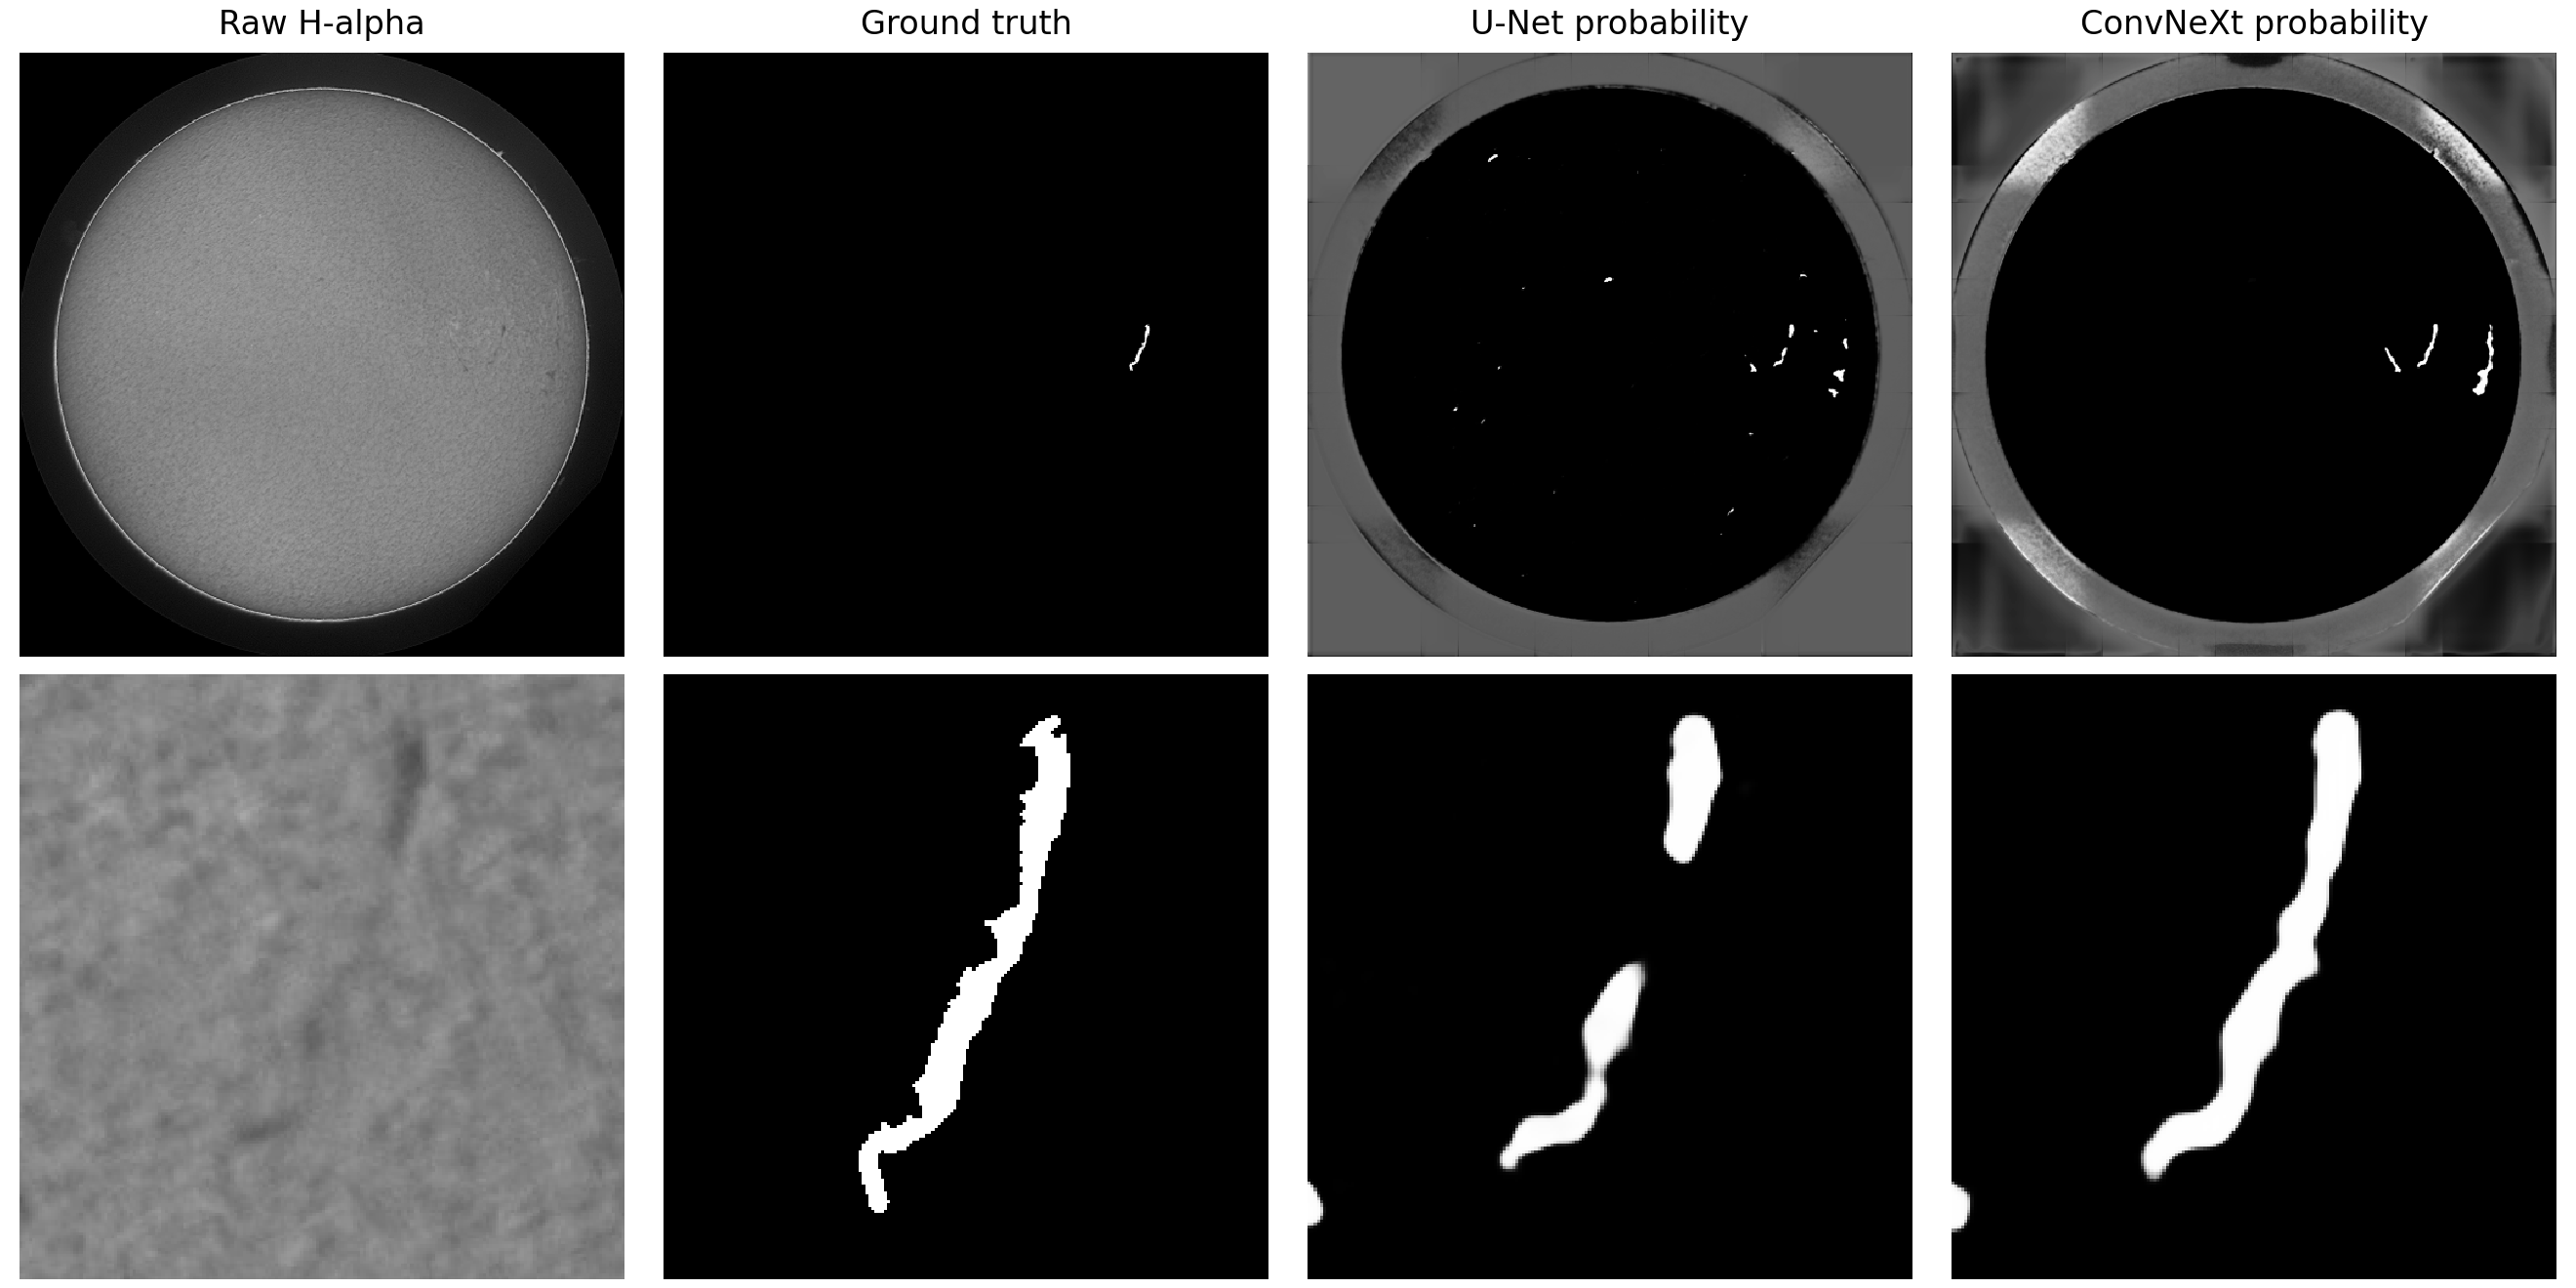
\includegraphics[width=\linewidth]{kaggle_qualitative.png}
\caption{Matched fold-0 view from the 16-epoch U-Net and ConvNeXt experiments, with a native-pixel detail crop.}
\label{fig:qualitative}
\end{figure}

\section{Limitations and remaining experiments}
All 27 CPU tests pass, including exact component-calibration statistics for overlapping and empty annotations. A running extension selects backbone weights and component hysteresis on fold 0, then evaluates saved-map subsets in folds 1--4. Subset results must remain separate from complete-fold measurements.

A separate completed refinement warm-started ConvNeXt folds 0 and 1 with 640-pixel native crops for 12 additional epochs of 600 samples, seed 142, learning rate $3\times10^{-5}$, and unchanged losses. Larger spatial context, added training, a restarted optimizer, and a new sample seed change together; this is an improvement experiment, not a crop-size ablation. Default extraction gives refinement PQ 0.3149 on all 249 fold-0 views and 0.1447 on all 215 fold-1 views, compared with 0.3355 and 0.3433 for the original ConvNeXt models. These uncalibrated results do not justify expansion. With component policies separately fitted on fold 0 and frozen, original and refined models obtain PQ 0.4049 and 0.4297 on the same 24 saved fold-1 annotation views, respectively. These limited-subset results were independently recomputed. A complete fold-1 comparison with those frozen policies and qualitative inspection is running before any expansion to other folds.

Residual atmospheric structure can bias radial normalization, and CLAHE can amplify noise. Boundary-based extraction can split one physical filament, while connected components can merge touching filaments. The three-day temporal rule requires sensitivity analysis against longer separations. Preprocessing ablations, longer temporal-separation checks, and inference-time measurements remain pending. The notebook now points to the exact submitted v1 source and frozen parameters. Its ten checkpoints remain in private Kaggle fold outputs and require download for portable reproduction. Public weight distribution and organizer-ready packaging remain unfinished; this document remains working notes.

\begin{thebibliography}{8}
\bibitem{magfilo} A. Ahmadzadeh, R. Adhyapak, K. Chaurasiya, et al., ``A dataset of manually annotated filaments from H-alpha observations,'' \emph{Scientific Data}, vol. 11, p. 1031, 2024, doi: 10.1038/s41597-024-03876-y.
\bibitem{magfiloweb} MLEcoFi, ``MAGFiLO: Manually Annotated GONG Filaments in H-Alpha Observations,'' \url{https://www.mlecofi.net/magfilo}, accessed Oct. 28, 2026.
\bibitem{challenge} A. Ahmadzadeh, D. J. Kempton, Q. Li, and A. A. Pevtsov, ``Solar Filament Segmentation Challenge 2026,'' Kaggle, 2026. \url{https://www.kaggle.com/competitions/filament-segmentation-2026}.
\bibitem{panoptic} A. Kirillov et al., ``Panoptic segmentation,'' in \emph{Proc. IEEE/CVF CVPR}, 2019, doi: 10.1109/CVPR.2019.00963.
\bibitem{segformer} E. Xie et al., ``SegFormer: Simple and efficient design for semantic segmentation with transformers,'' in \emph{NeurIPS}, 2021, arXiv:2105.15203.
\bibitem{convnext} Z. Liu et al., ``A ConvNet for the 2020s,'' in \emph{Proc. IEEE/CVF CVPR}, 2022, arXiv:2201.03545.
\bibitem{unetpp} Z. Zhou et al., ``UNet++: A nested U-Net architecture for medical image segmentation,'' \emph{DLMIA/ML-CDS}, 2018, arXiv:1807.10165.
\bibitem{cldice} S. Shit et al., ``clDice: A novel topology-preserving loss function for tubular structure segmentation,'' in \emph{Proc. IEEE/CVF CVPR}, 2021, arXiv:2003.07311.
\end{thebibliography}
\end{document}
